% Useful Tools for Recording Bioinformatics Work
%
% Subsection listing several tools that are useful for recording bioinformatics work

\subsection{Useful Tools for Recording Bioinformatics Work}
\begin{frame}
  \frametitle{Plain Text Files}
  \begin{itemize}
    \item \texttt{README.txt}/\texttt{README.md} in each directory/folder
    \item Plain text is always human-readable
    \begin{itemize}
      \item Markdown (\url{https://daringfireball.net/projects/markdown/basics})
      \item RST (\url{http://docutils.sourceforge.net/docs/ref/rst/restructuredtext.html})
    \end{itemize}
  \end{itemize}
  \begin{center}
    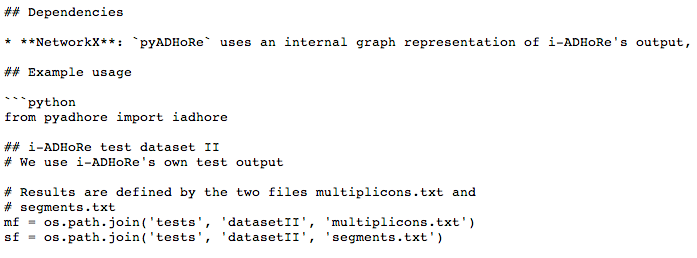
\includegraphics[width=.4\textwidth]{images/markdown_before}
    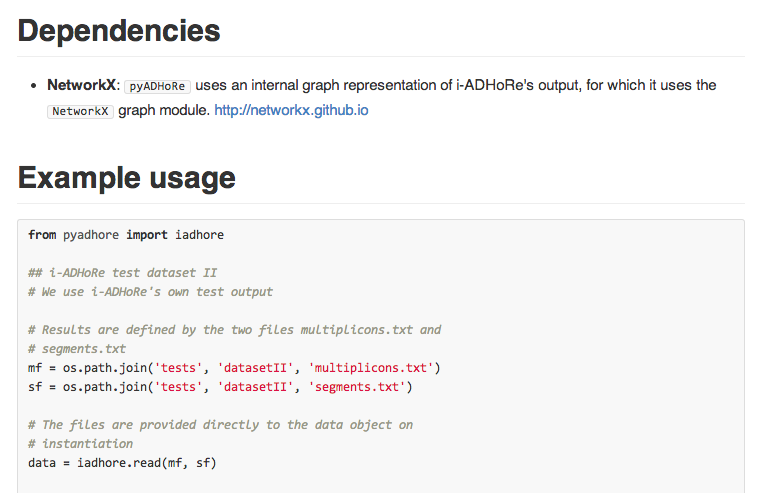
\includegraphics[width=.4\textwidth]{images/markdown_after}
  \end{center}
\end{frame}
   
\begin{frame}
  \frametitle{Galaxy workflows}
  \begin{itemize}
    \item Use through browser, graphical interface
    \item Reproducible, shareable, documentable, reusable analyses
    \item Wraps standard bioinformatics tools
    \item Local instance (\url{http://galaxy.hutton.ac.uk}) uses JHI cluster       
  \end{itemize}
  \begin{center}
    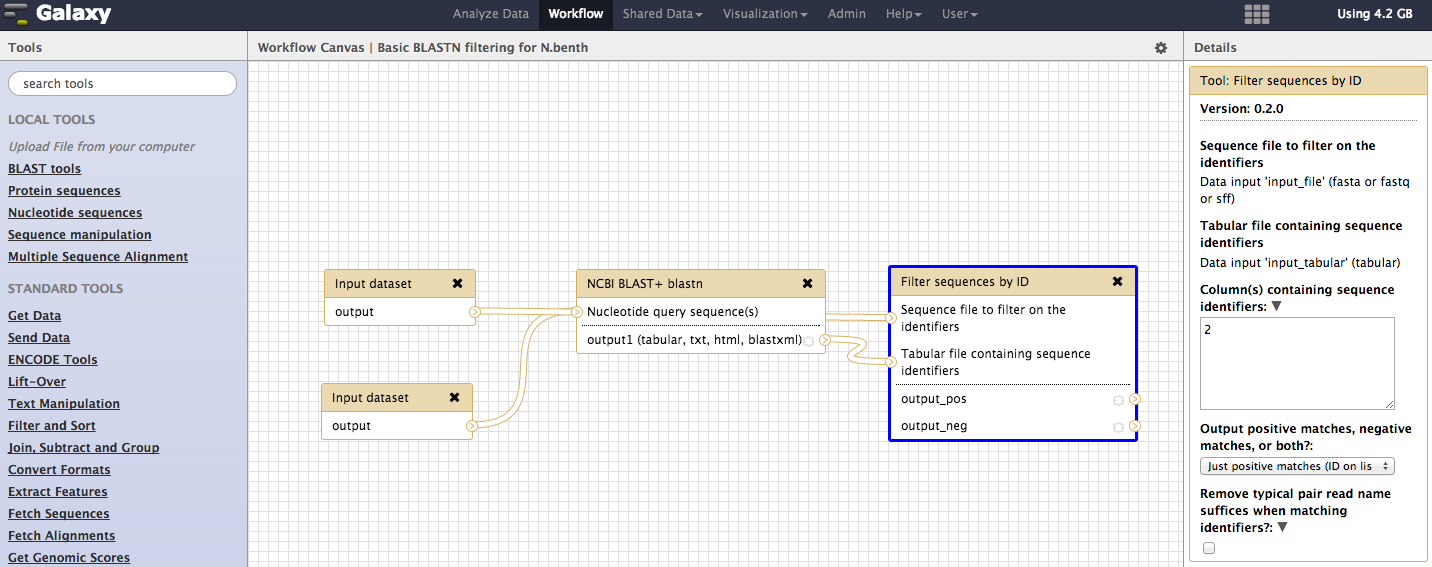
\includegraphics[width=.75\textwidth]{images/galaxy_screenshot}
  \end{center}
\end{frame}      

\begin{frame}
  \frametitle{A language notebook}
  \begin{itemize}
    \item e.g. \texttt{iPython Notebook}, \texttt{knitr}, \texttt{Mathematica}, \texttt{MatLab} cells
    \item Integrates live code and analysis with lab-book
  \end{itemize}
  \begin{center}
    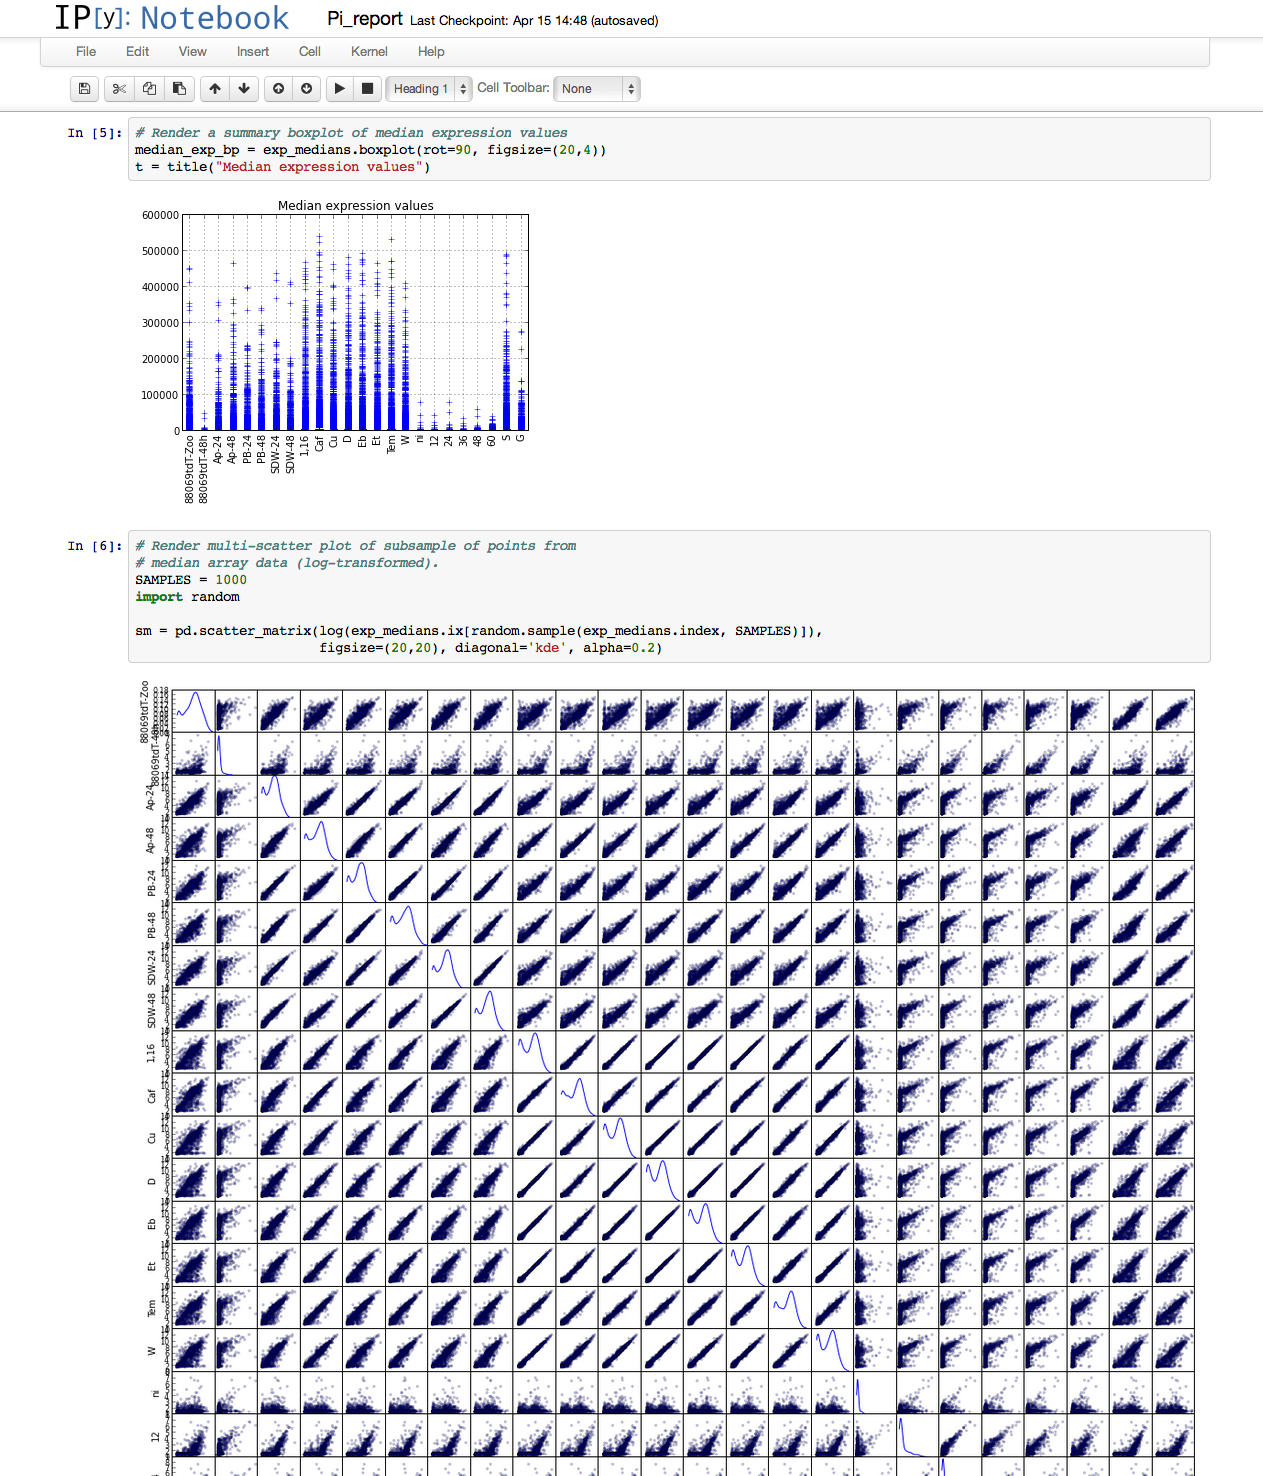
\includegraphics[width=.35\textwidth]{images/ipython_notebook}     
  \end{center}
\end{frame}
